\documentclass{../../slides-style}

\slidetitleext{Лекция 11: Сопровождение и реинжиниринг}{02.05.2023}{Сопровождение и реинжиниринг}

\begin{document}

    \begin{frame}[plain]
        \titlepage
    \end{frame}

    \section{Динамика развития программ}

    \begin{frame}
        \frametitle{Сопровождение}
        \begin{outline}
            \1 Сопровождение неизбежно:
                \2 Развитие бизнес-процессов
                \2 Изменение внешнего окружения
                \2 Исправление ошибок
                \2 Повышение производительности
            \1 Организации зависят от ПО
                \2 Иногда критически
            \1 Сопровождение стоит денег и усилий
        \end{outline}
    \end{frame}

    \begin{frame}
        \frametitle{Законы Лемана}
        \begin{outline}
            \1 Непрерывное изменение
            \1 Увеличение сложности
            \1 Саморегулирование
            \1 Сохранение организационной стабильности
            \1 Сохранение осведомлённости
            \1 Ухудшение качества
            \1 Система обратной связи
        \end{outline}
    \end{frame}

    \section{Унаследованные системы}

    \begin{frame}
        \frametitle{Унаследованные (legacy) системы}
        \begin{outline}
            \1 Жизненный цикл --- 20 лет и более
            \1 Высокие риски при замене
                \2 Нет технического описания
                \2 Система переплетена с бизнес-процессами
                \2 Система является единственным источником знаний о некоторых бизнес-правилах
                    \3 Включая ошибки системы!
                \2 Риски разработки новой системы
        \end{outline}
    \end{frame}

    \begin{frame}
        \frametitle{Стоимость поддержки}
        \begin{outline}
            \1 Разные команды $\to$ разный стиль
            \1 Устаревшие технологии $\to$ сложно искать кадры
            \1 Качество и актуальность документации
                \2 Иногда её просто нет
                \2 Иногда нет даже кода
            \1 Архитектурная эрозия
            \1 Оптимизации
            \1 Дублирование и неконсистентность данных
        \end{outline}
    \end{frame}

    \begin{frame}
        \frametitle{Что делать?}
        \begin{center}
            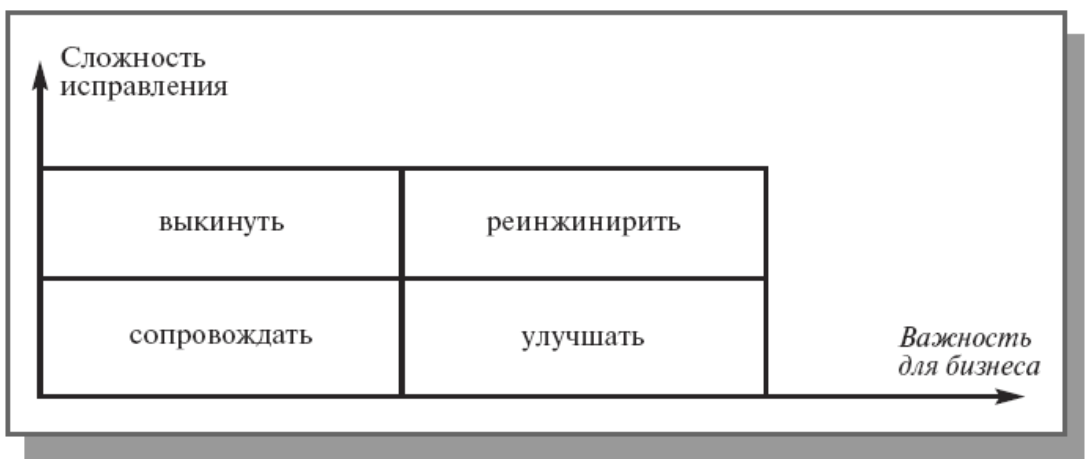
\includegraphics[width=0.7\textwidth]{maintenanceWays.png}
        \end{center}
    \end{frame}

    \section{Модернизация программного обеспечения}

    \begin{frame}
        \frametitle{Модернизация программного обеспечения}
        \begin{outline}
            \1 Учитывать важность для бизнеса
            \1 Учитывать качество
            \1 Учитывать аппаратное обеспечение и окружение
            \1 К разным частям системы могут применяться разные стратегии
                \2 К разным программам в составе системы --- тем более
        \end{outline}
    \end{frame}

    \subsection{Сопровождение}

    \begin{frame}
        \frametitle{Сопровождение}
        \begin{outline}
            \1 Исправление ошибок
            \1 Адаптация к условиям эксплуатации
            \1 Изменение функциональности
            \1 Профилактическое сопровождение
        \end{outline}
        \pause
        \vspace{5mm}
        \begin{outline}
            \1 65\% --- выполнение новых требований
            \1 18\% --- адаптация к новому окружению
            \1 17\% --- исправление ошибок
        \end{outline}
    \end{frame}

    \begin{frame}
        \frametitle{Факторы стоимости сопровождения}
        \begin{outline}
            \1 Стабильность команды разработчиков
            \1 Ответственность согласно контракту
                \2 Оригинальные разработчики не мотивированы облегчить сопровождение
            \1 Квалификация специалистов
            \1 Возраст и структура программы
        \end{outline}
    \end{frame}

    \begin{frame}
        \frametitle{Процесс сопровождения}
        \begin{center}
            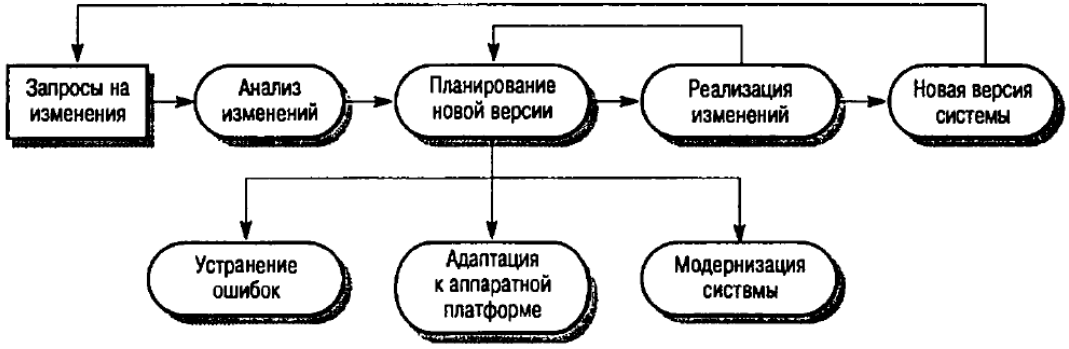
\includegraphics[width=0.9\textwidth]{maintenanceProcess.png}
        \end{center}
    \end{frame}

    \begin{frame}
        \frametitle{Нарушения процесса}
        \begin{outline}
            \1 Часто бывает нужно
                \2 Критическая ошибка в системе
                \2 Изменение рабочего окружения
                \2 Неожиданные изменения бизнеса
                    \3 Например, изменения законодательства
            \1 Потеря целостности требований и архитектуры
            \1 Выбор быстрого решения, а не правильного
                \2 Откатить хотфикс и <<сделать нормально>>
        \end{outline}
    \end{frame}

    \begin{frame}
        \frametitle{Прогнозирование сопровождения}
        \begin{outline}
            \1 Количество и сложность интерфейсов
            \1 Количество изменяемых системных требований
            \1 Бизнес-процессы, в которых используется данная система
            \1 Взаимосвязанность и сложность компонентов
                \2 Вспомним лекцию про метрики
        \end{outline}
    \end{frame}

    \begin{frame}
        \frametitle{Оценка удобства сопровождения}
        \begin{outline}
            \1 Количество запросов на корректировку системы
            \1 Количество корректировок, которые затронули каждый модуль
            \1 Среднее время, потраченное на анализ причин системных сбоев и отказов
            \1 Среднее время, необходимое на реализацию изменений
            \1 Количество незавершенных запросов на изменения
        \end{outline}
    \end{frame}

    \begin{frame}
        \frametitle{Личные качества сопровождающего программиста}
        \begin{outline}
            \1 Гибкость в работе
            \1 Творческий подход к задачам
            \1 Широкий профессиональный кругозор
            \1 Хорошая память
            \1 Терпение
            \1 Самостоятельность
            \1 Ответственность и самокритичность
        \end{outline}
    \end{frame}

    \subsection{Техподдержка}

    \begin{frame}
        \frametitle{Техподдержка, виды контрактов}
        \begin{outline}
            \1 Фиксированный объём работ
            \1 Техподдержка на определённый срок
            \1 Поддержка по необходимости (Time and Materials)
            \1 Сопровождение продукта
        \end{outline}
    \end{frame}

    \begin{frame}
        \frametitle{Линии поддержки}
        \begin{outline}
            \1 Линия 1 --- сбор информации, решение проблем по FAQ
                \2 Неквалифицированные кадры, не решают технические проблемы
            \1 Линия 2 --- помощь линии 1, решение известным способом
                \2 Специалисты, разбирающиеся в продукте
                \2 Некоторая техническая работа, типа правки данных
                \2 Может быть несколько специализированных групп
            \1 Линия 3 --- решение неизвестных проблем
                \2 Настоящая команда сопровождения/разработки
        \end{outline}
    \end{frame}

    \subsection{Улучшение}

    \begin{frame}
        \frametitle{Улучшение}
        \framesubtitle{Как работать с унаследованным кодом}
        \begin{outline}
            \1 Понимать, что код уже приносит прибыль
                \2 Каким бы плохим он ни был, он лучше ненаписанного
                \2 Ответственность
            \1 Reverse engineering
                \2 Восстановление архитектуры
                \2 Отслеживание цепочек вызовов
                \2 Исследовательская отладка
                \2 Промышленная археология
                \2 Документирование результатов
        \end{outline}
    \end{frame}

    \begin{frame}
        \frametitle{Советы по процессу}
        \begin{outline}
            \1 Не переписывайте код
            \1 Не меняйте технологии/парадигму
                \2 Но есть распределённые приложения
            \1 Помните о бизнес-интересах
            \1 Не забывайте про логирование
            \1 Не забывайте про тестирование
                \2 Characterization testing
            \1 Постройте чёткий процесс релизов
            \1 Определите стратегию версионирования кода
            \1 Контролируйте качество кода
                \2 Code review
            \1 Выделяйте (и переписывайте) отдельные модули
        \end{outline}
    \end{frame}

    \begin{frame}
        \frametitle{<<Приложение-душитель>>}
        \begin{center}
            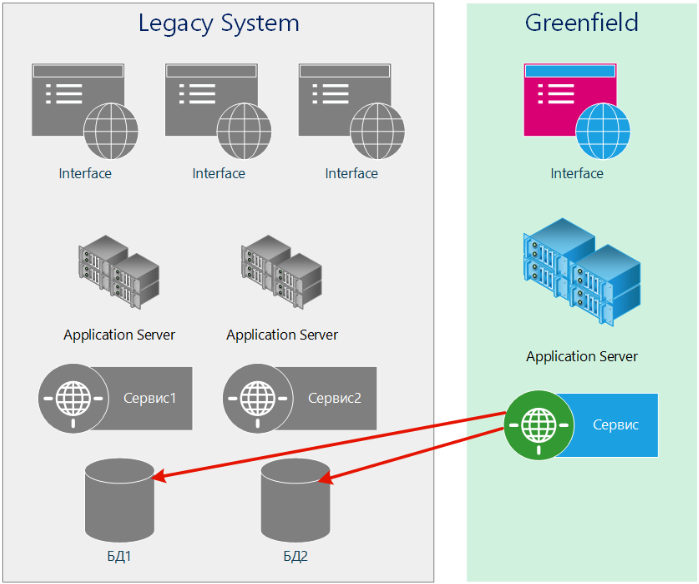
\includegraphics[width=0.6\textwidth]{stranglerApp.png}
        \end{center}
    \end{frame}

    \section{Реинжиниринг}

    \begin{frame}
        \frametitle{Реинжиниринг}
        \begin{center}
            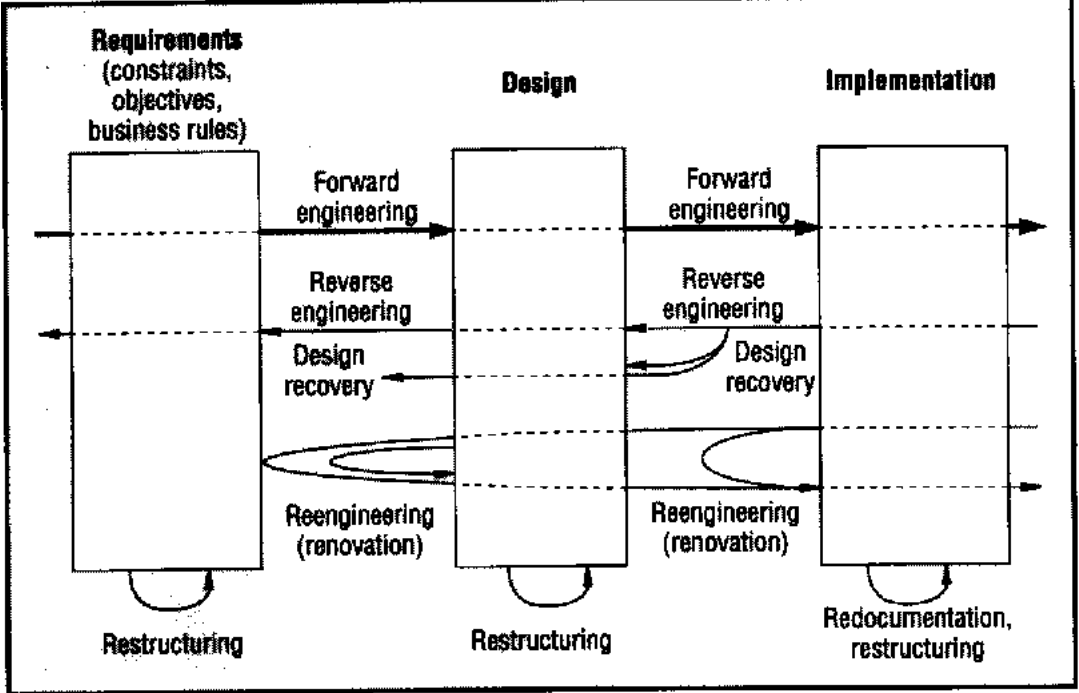
\includegraphics[width=0.8\textwidth]{reengineering.png}
            \attribution{E. Chikofsky et al. Reverse engineering and design recovery: a taxonomy}
        \end{center}
    \end{frame}

    \begin{frame}
        \frametitle{Реинжиниринг против полного переписывания}
        \begin{outline}
            \1 Унаследованного кода очень много
                \2 120 млрд строк на 1990 год, и это было только начало
            \1 Снижение рисков
            \1 Снижение затрат
                \2 Примерно в четыре раза дешевле, чем разработка с нуля
                \2 Автоматизируем
            \1 Ограничен в возможностях улучшения системы
                \2 Только частично решает проблему сопровождения
        \end{outline}
    \end{frame}

    \begin{frame}
        \frametitle{Реинжиниринг против полного переписывания}
        \begin{center}
            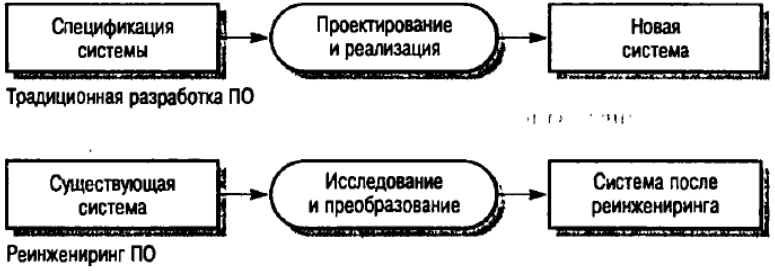
\includegraphics[width=0.7\textwidth]{developmentVsReengineering.png}
        \end{center}
    \end{frame}

    \begin{frame}
        \frametitle{Стоимость реинжиниринга}
        \begin{center}
            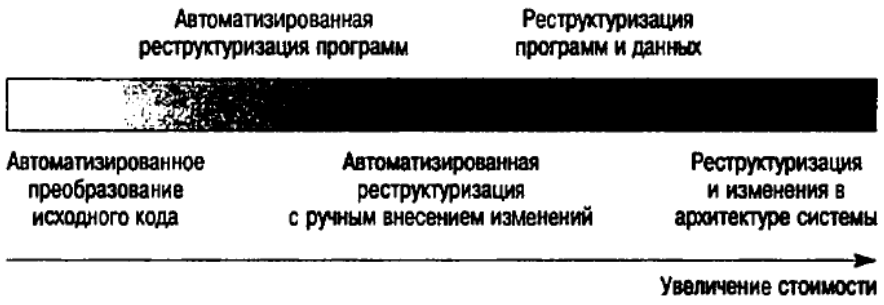
\includegraphics[width=0.7\textwidth]{reengineeringAutomation.png}
        \end{center}
    \end{frame}

    \begin{frame}
        \frametitle{Факторы стоимости}
        \begin{outline}
            \1 Качество программного обеспечения, которое подвергается реинжинирингу
            \1 Наличие средств поддержки процесса реинжиниринга
            \1 Объем необходимого преобразования данных
            \1 Наличие необходимых специалистов
        \end{outline}
    \end{frame}

    \begin{frame}
        \frametitle{Процесс реинжиниринга}
        \begin{center}
            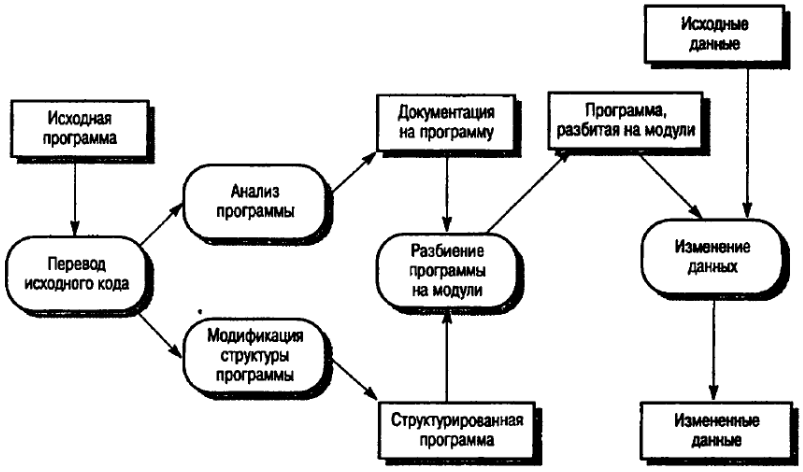
\includegraphics[width=0.8\textwidth]{reengineeringProcess.png}
        \end{center}
    \end{frame}

    \begin{frame}
        \frametitle{Перевод исходного кода}
        \begin{center}
            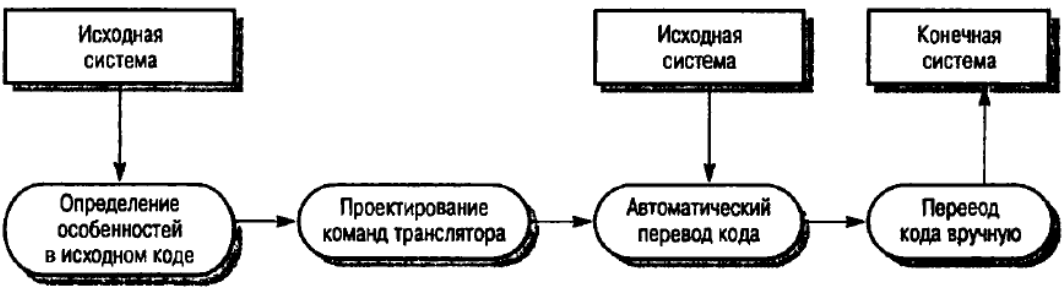
\includegraphics[width=0.8\textwidth]{sourceCodeTranslation.png}
        \end{center}
    \end{frame}

    \begin{frame}
        \frametitle{Анализ программ}
        \begin{center}
            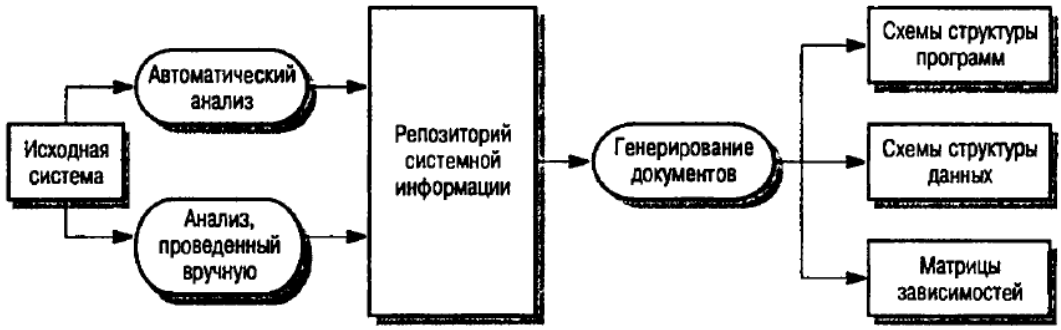
\includegraphics[width=0.8\textwidth]{programStructureAnalysis.png}
        \end{center}
    \end{frame}

    \begin{frame}
        \frametitle{Модификация структуры программ}
        \begin{center}
            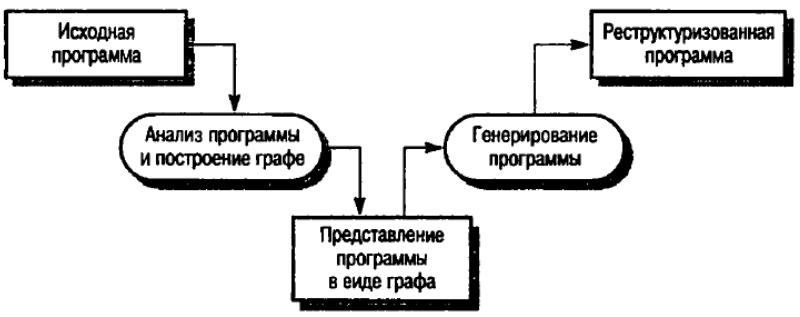
\includegraphics[width=0.7\textwidth]{programStructureReengineering.png}
        \end{center}
    \end{frame}

    \begin{frame}
        \frametitle{Автоматизация}
        \begin{outline}
            \1 Инвентаризация исходного кода
            \1 Разбор исходного кода
            \1 Выделение графов потока управления, потока данных
            \1 Анализ потока управления, потока данных
            \1 Удаление мёртвого кода, извлечение бизнес-правил
            \1 Генерация АСД целевого языка
                \2 Переписыватели деревьев, например, Stratego/XT
            \1 Генерация кода и правил сборки
        \end{outline}
    \end{frame}

    \begin{frame}
        \frametitle{Автоматизация, проблемы}
        \begin{outline}
            \1 Потеря комментариев
                \2 Зависит от используемого инструмента
            \1 Утрата связи с документацией
                \2 Скорее всего, она всё равно устарела
            \1 Жесткие требования к компьютерной технике
                \2 Зависит от используемого инструмента
        \end{outline}
    \end{frame}

    \begin{frame}
        \frametitle{Разбиение на модули}
        \begin{outline}
            \1 Реинжинирить только нужное:
                \2 Интенсивность сбоев
                \2 Частота изменений
                \2 Сложность
                    \3 Метрики!
            \1 Явное вынесение модулей
                \2 Абстракции данных
                \2 Аппаратные модули
                \2 Функциональные модули
                \2 Модули поддержки отдельных процессов
            \1 Делается вручную
        \end{outline}
    \end{frame}

    \begin{frame}
        \frametitle{Изменение данных}
        \begin{outline}
            \1 Критично для информационных систем
            \1 Причины изменений:
                \2 Нарушение данных
                    \3 Дублирование и неконсистентность
                    \3 Долгие сроки хранения и устаревание
                \2 Программные ограничения
                    \3 Кто помнит телефоны <<не более 100 SMS>>?
                \2 Эволюция системной архитектуры
                    \3 Распределённые системы
            \1 Требуется анализ кода на литералы
        \end{outline}
    \end{frame}

    \begin{frame}
        \frametitle{Модификация структуры программ}
        \begin{center}
            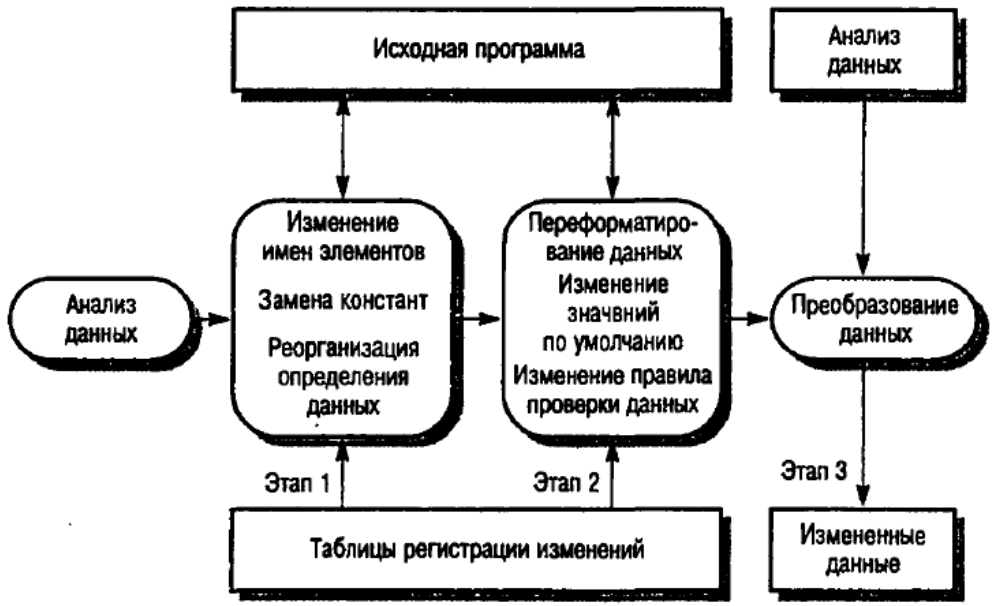
\includegraphics[width=0.75\textwidth]{dataReengineering.png}
        \end{center}
    \end{frame}

\end{document}